% 图 24.2 —— 由 `checks/emit_hand.py` 自动拼出（probe 精测 + prims2 图元分解）
%%
% ⚠ 这是**稿子不是成品**：跑 `checks/checkhand.py 24.2` 看指标 + 看叠合图。
%%
%% ⚠ 待核：
%   · 本图 probe 报出阴影族 1 个 —— **本脚本不生成阴影**（要照原书手写）；prims2 的 strokes 里可能含阴影线，核对时留意别画重
%   · 可疑字形 1 项（空心圈 ⊙ 常被认成字母 o）—— 见文件末
%%
\documentclass[12pt]{standalone}
\usepackage{fontspec}
\setsansfont{Arial}
\newfontfamily\mfallback{DejaVu Sans}
\usepackage{tikz}
\begin{document}
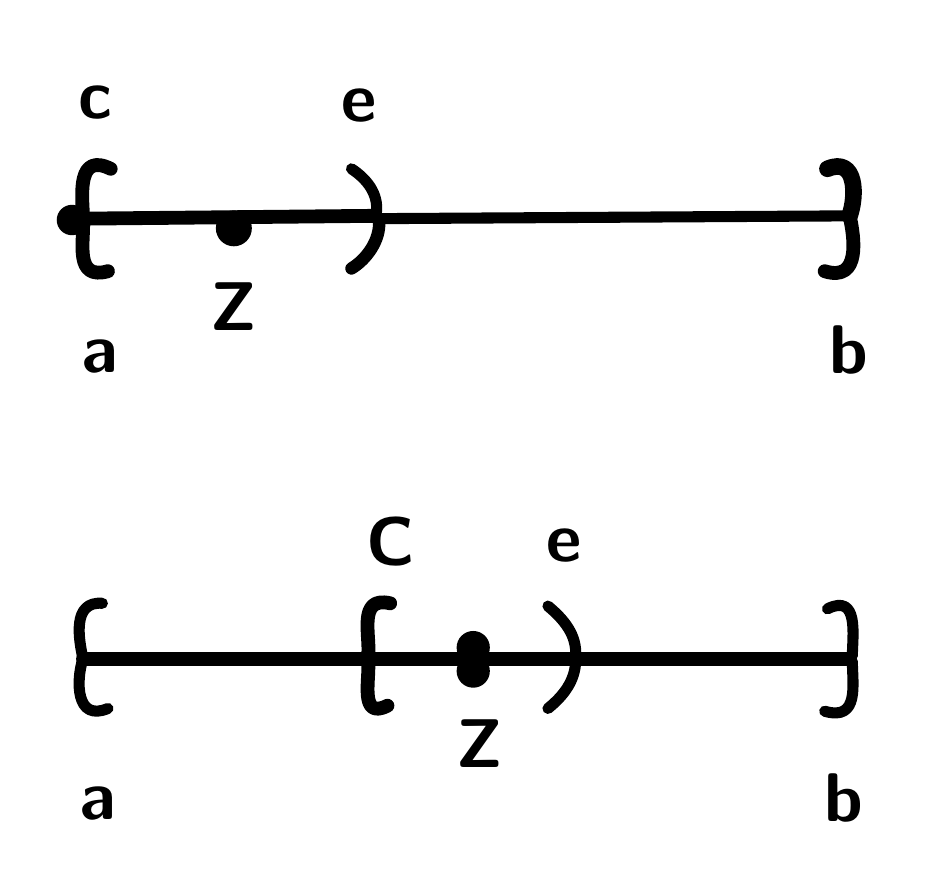
\begin{tikzpicture}[x=1pt, y=-1pt, line width=5.0pt, line cap=round, line join=round]

  %% ════ 填充区（prims2 的 fills）════

  %% ════ 直线段（prims2 的 strokes）════
  \draw[line width=5.0pt] (122.0,228.0) -- (20.0,228.0);
  \draw[line width=4.0pt] (128.0,69.0) -- (297.0,68.0);
  \draw[line width=5.0pt] (124.0,228.0) -- (197.0,228.0);
  \draw[line width=5.0pt] (21.0,69.0) -- (125.0,68.0);
  \draw[line width=5.0pt] (297.0,228.0) -- (199.0,228.0);

  %% ════ 曲线（prims2 的 curves —— 三段式，坐标同为 (y,x)）════
  \draw[line width=4.0pt] (126.0,67.0) .. controls (126.9,60.0) and (122.5,54.6) .. (117.0,51.0);
  \draw[line width=4.0pt] (298.0,229.0) .. controls (298.0,237.1) and (300.7,250.7) .. (288.0,247.0);
  \draw[line width=4.0pt] (188.0,209.0) .. controls (193.8,213.8) and (198.5,219.5) .. (198.0,227.0);
  \draw[line width=5.0pt] (123.0,227.0) .. controls (124.0,220.0) and (119.0,205.2) .. (131.0,208.0);
  \draw[line width=5.0pt] (20.0,68.0) .. controls (19.6,60.2) and (17.9,45.0) .. (30.0,51.0);
  \draw[line width=5.0pt] (29.0,88.0) .. controls (16.8,91.4) and (20.4,77.4) .. (20.0,70.0);
  \draw[line width=4.5pt] (127.0,70.0) .. controls (127.4,76.8) and (122.5,83.7) .. (117.0,87.0);
  \draw[line width=5.0pt] (288.0,88.0) .. controls (301.2,92.1) and (298.7,75.6) .. (297.0,68.0);
  \draw[line width=4.0pt] (188.0,246.0) .. controls (193.6,241.5) and (197.8,236.0) .. (198.0,229.0);
  \draw[line width=5.0pt] (123.0,229.0) .. controls (123.8,234.9) and (119.6,250.3) .. (130.0,245.0);
  \draw[line width=4.0pt] (27.0,208.0) .. controls (16.0,207.1) and (18.4,220.9) .. (20.0,228.0);
  \draw[line width=6.0pt] (297.0,68.0) .. controls (299.5,60.9) and (299.7,46.5) .. (289.0,51.0);
  \draw[line width=4.0pt] (29.0,246.0) .. controls (17.3,251.0) and (17.4,235.8) .. (20.0,228.0);
  \draw[line width=4.0pt] (289.0,210.0) .. controls (300.6,204.2) and (298.0,220.0) .. (298.0,227.0);

  %% ════ 实心点 ════
  \fill (16.0,69.5) circle (5.5);
  \fill (74.5,72.5) circle (6.5);
  \fill (161.0,224.0) circle (6.0);
  \fill (161.0,232.5) circle (6.0);

  %% ════ 标签（probe 直接给的 \node 行）════
  %% ⚠ 全部补了 fill=white：文字在最上层，否则与曲线交叉干扰
     \node[anchor=center,inner sep=0pt,fill=white,font=\fontsize{30.5}{38.1}\selectfont] at (24.3,27.0) {\textsf{\textbf{\textit{c}}}};   % box(16,17,15,17)
     \node[anchor=center,inner sep=0pt,fill=white,font=\fontsize{31.4}{39.3}\selectfont] at (119.8,28.1) {\textsf{\textbf{\textit{e}}}};   % box(110,18,16,17)
     \node[anchor=center,inner sep=0pt,fill=white,font=\fontsize{23.7}{29.7}\selectfont] at (74.4,100.8) {\textsf{\textbf{\textit{Z}}}};   % box(65,92,16,16)
     \node[anchor=center,inner sep=0pt,fill=white,font=\fontsize{30.0}{37.5}\selectfont] at (296.8,116.2) {\textsf{\textbf{\textit{b}}}};   % box(287,104,17,22)
     \node[anchor=center,inner sep=0pt,fill=white,font=\fontsize{31.0}{38.7}\selectfont] at (26.5,119.0) {\textsf{\textbf{\textit{a}}}};   % box(18,109,15,17)
     \node[anchor=center,inner sep=0pt,fill=white,font=\fontsize{23.4}{29.3}\selectfont] at (131.1,185.7) {\textsf{\textbf{\textit{C}}}};   % box(123,177,15,17)
     \node[anchor=center,inner sep=0pt,fill=white,font=\fontsize{31.4}{39.3}\selectfont] at (193.8,187.1) {\textsf{\textbf{\textit{e}}}};   % box(184,177,16,17)
     \node[anchor=center,inner sep=0pt,fill=white,font=\fontsize{23.7}{29.7}\selectfont] at (163.4,258.8) {\textsf{\textbf{\textit{Z}}}};   % box(154,250,16,16)
     \node[anchor=center,inner sep=0pt,fill=white,font=\fontsize{30.0}{37.5}\selectfont] at (294.8,278.2) {\textsf{\textbf{\textit{b}}}};   % box(285,266,17,22)
     \node[anchor=center,inner sep=0pt,fill=white,font=\fontsize{30.0}{37.6}\selectfont] at (25.5,280.5) {\textsf{\textbf{\textit{a}}}};   % box(17,271,15,16)

  % 钉死画布：否则超出的图元/控制点会把页面撑大，1:1 回比就失准
  \pgfresetboundingbox
  \path[use as bounding box] (0,0) rectangle (314,295);
\end{tikzpicture}
\end{document}

% ⚠ 待核清单（probe 拿不准，人眼过一遍）：
%   · 未识别/跳过：⑤ 跳过/未识别的字形
